\subsection{Intensity}

The minimum MSLP found in the track and best track was plotted as Central Pressure in Figure \ref{fig:monera5} (a). The forecasted wind at the first model level alongside with the maximum wind speed of best track and the 10 meters instantaneous gust-front of ERA5 are displayed in Figure \ref{fig:monera5} (b). The Saffir-Simpson wind scale is denoted by black lines to guide the reader in the forecast scale. 

\begin{figure}[!ht]
	\centering
	\caption{Comparison of Forecasted and Observed Central Pressure and Wind Speeds for Hurricane Beryl. Here, a 12-hour model spin-up was also withdrawn, starting the time series on July 3rd, 12 UTC.} % Título acima da figura
	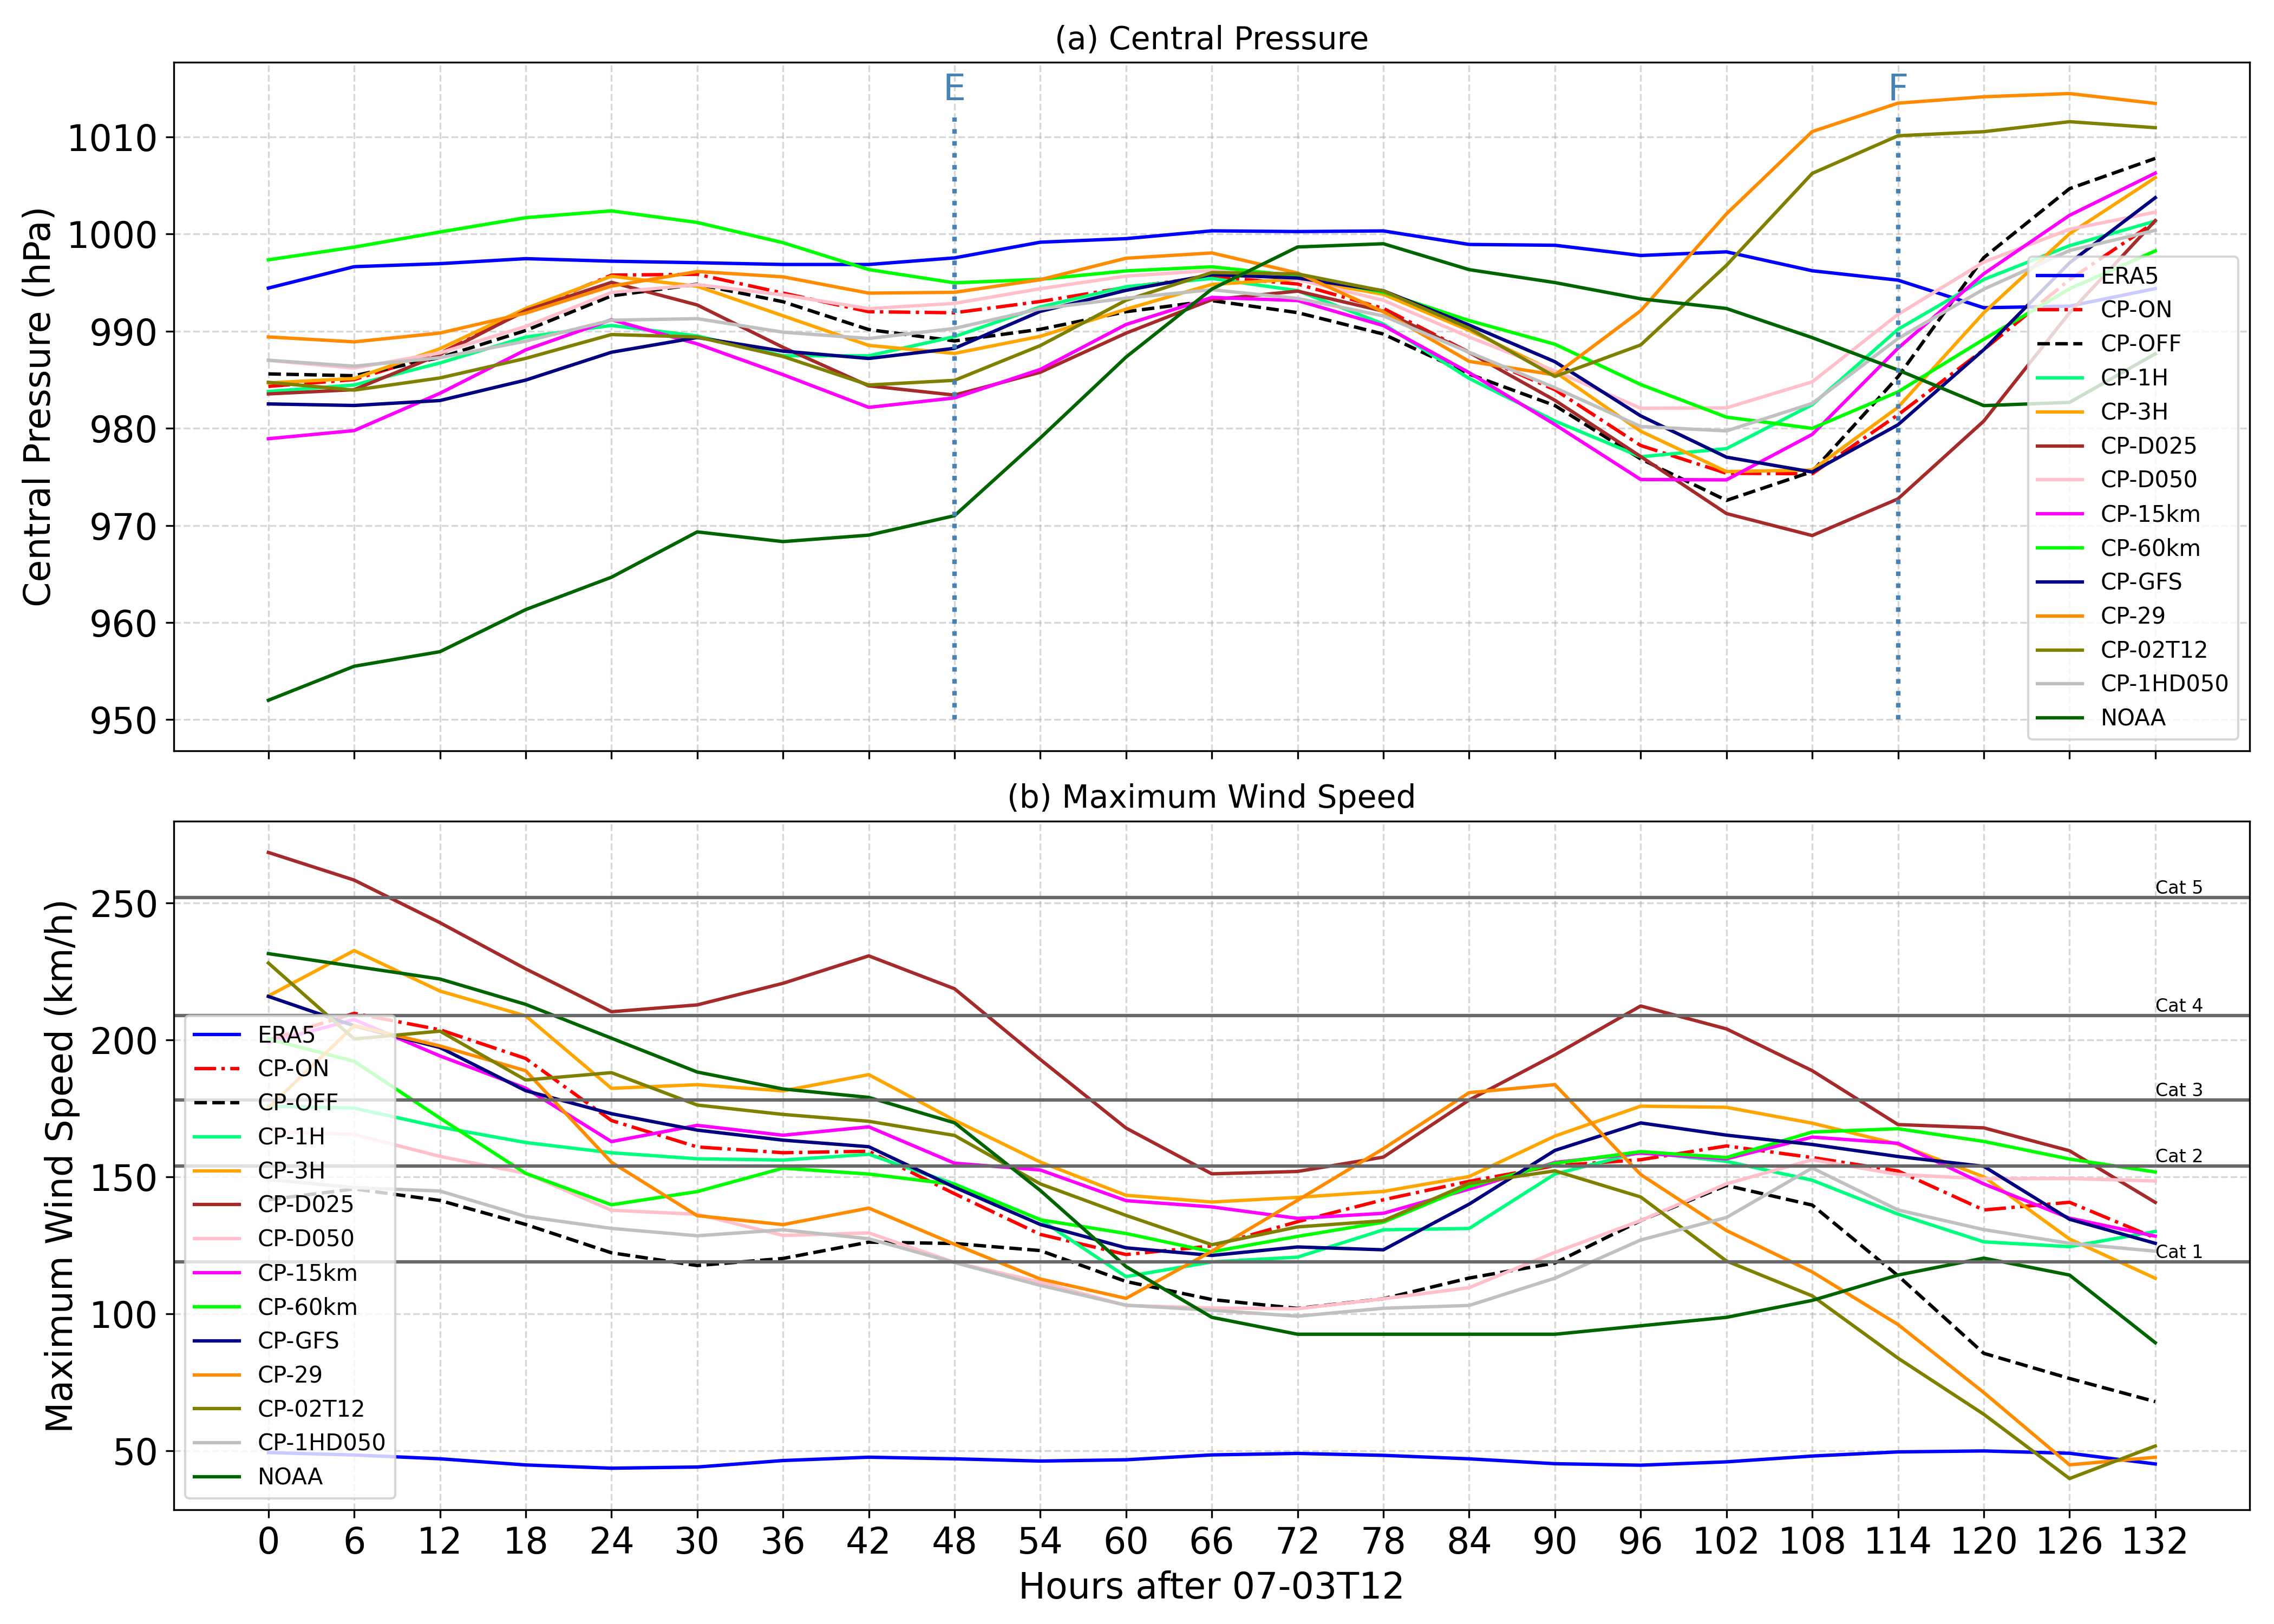
\includegraphics[width=\textwidth]{docs/figuras/chapter5/intensity_time_series_panel_FINAL.png} 
	\vspace{0.5em}
	Source: Made by the author (2025).  % Fonte abaixo da imagem
	\label{fig:monera5} % Label para referenciar no texto
\end{figure}

In general, this panel indicates that the ERA5 reanalysis demonstrates poorer performance in predicting central pressure compared to MONAN forecasts. This finding aligns with the work of \citeonline{dulac2024assessing}, who highlight that inaccuracies in central pressure estimations can lead to underestimations in wind speed intensity predictions. Given that MONAN is initialized with ERA5 reanalysis fields, it is anticipated that the initial conditions also carry those uncertainties.

As shown in Figure \ref{fig:monera5} (a), the MONAN forecasts exhibit a similar trend; however, there are notable outliers, particularly in the CP-29 and CP-02T12 experiments, especially following the Texas entrance (marked by the vertical line "F").

The initial high-pressure peak occurring between 24 and 30 hours of the forecast is in phase with the best track. However, after the passage of the Yucatan Peninsula, at 66-72 hours of forecast, the experiments fall out of phase by approximately 6 hours, with MONAN displaying an earlier peak than the best track. A forecasted low-pressure system intensifies around 102-108 hours, while the best track identifies this feature closer to 126 hours. This behavior is consistent with what the ATE indicated earlier.

The cold pool effect is most noticeable in Figure \ref{fig:monera5} (b). The CP-ON configuration tends to generate more wind than CP-OFF, yet it does not reach the strength reported in the best track data.

The forecasts initialized earlier than the standard (CP-29 and CP-02T12) in Figure \ref{fig:monera5}  (b) also emerge as outliers. This discrepancy becomes particularly evident when we examine the last intensification moment from the best track, at 120 hours, achieving Category 1. In contrast, these forecasts peak at 90 hours, showing even greater intensity as they reach Categories 2 and 3. This indicates a significant divergence of a full day between these forecasts and the intensity described by the best track. This trend, consistent with the observations in the ATE, is also reflected in the other forecasts. Furthermore, the anticipation of peak intensity worsens as the integration time extends.

One of the most striking forecasts in this figure is from the CP-D025 experiment, which illustrates an excessively intense system. This intensity arises because the mass flux is situated much closer to the surface compared to the other experiments, resulting in stronger downdrafts and, consequently, a more intense gust.

The panel presents a quantitative evaluation of the forecasts and ERA5 reanalysis in comparison to the intensity observed in the best track. The RMSE in these figures is a particularly insightful metric due to the oscillatory nature of the event, as this error is computed as a weighted average of the squared differences.

\begin{figure}[!ht]
	\centering
	\caption{Central Pressure and Maximum Wind Speed Errors.} % Título acima da figura
	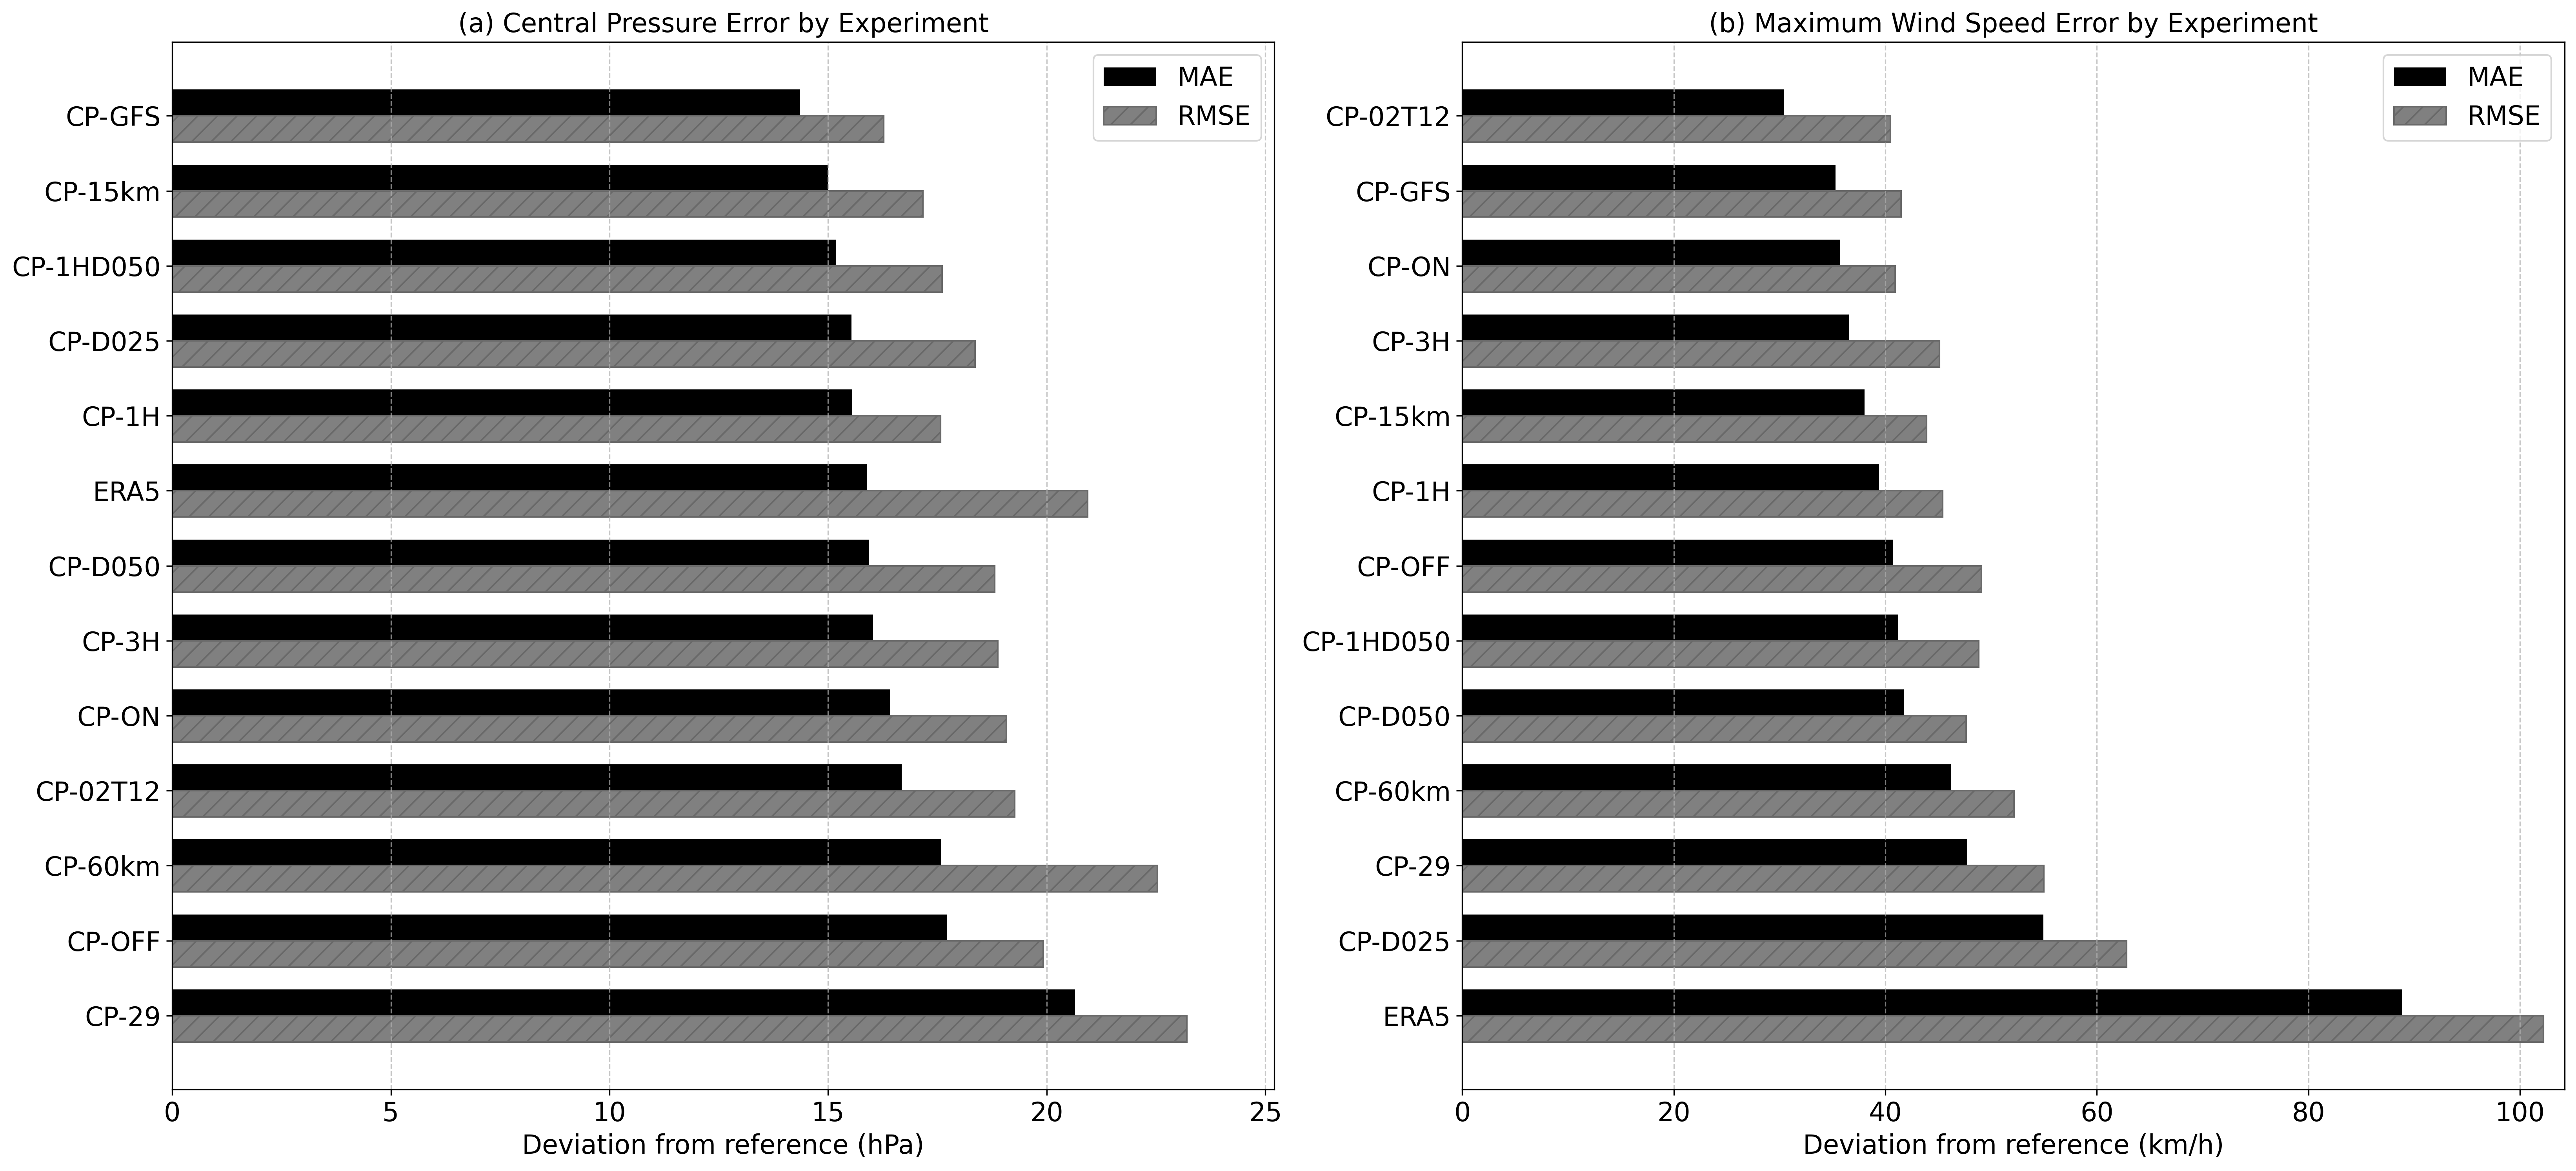
\includegraphics[width=\textwidth]{docs/figuras/chapter5/panel_mae_rmse_mslp_wspd_FINAL.png} 
	\vspace{0.5em}
	Source: Made by the author (2025).  % Fonte abaixo da imagem
	\label{fig:errors} % Label para referenciar no texto
\end{figure}

In Figure \ref{fig:errors} (a), the performance of the cold pools in the pressure field is evident, with CP-ON showing a reduction in MAE of approximately 8\% compared to CP-OFF. Furthermore, the importance of investigating and tuning the parameters within this parametrization is highlighted, as modifying them leads to further improvements in pressure representation. Notably, the CP-1HD050 configuration stands out, despite not achieving the same improvement in the wind field. This relationship between cold pools and the pressure field could be further explored in future studies.

In Figure \ref{fig:errors} (b), it is interesting to note that CP-ON reduces the MAE by approximately 12.5\% compared to CP-OFF, while the RMSE shows an even greater reduction of about 20\%. Although the CP-D025 experiment produces a system that is too intense, diverging from the best track, as shown in the previous figure, it does not result in a worsening of the pressure field, once again underscoring the importance of parameter tuning within the convection scheme.

By the end, a mean of Figure \ref{fig:errorsmona} is presented next, to highlight the differences between ERA5 and MONAN.

\begin{figure}[!ht]
	\centering
	\caption{Central Pressure and Maximum Wind Speed errors by MONAN compared to ERA5.} % Título acima da figura
	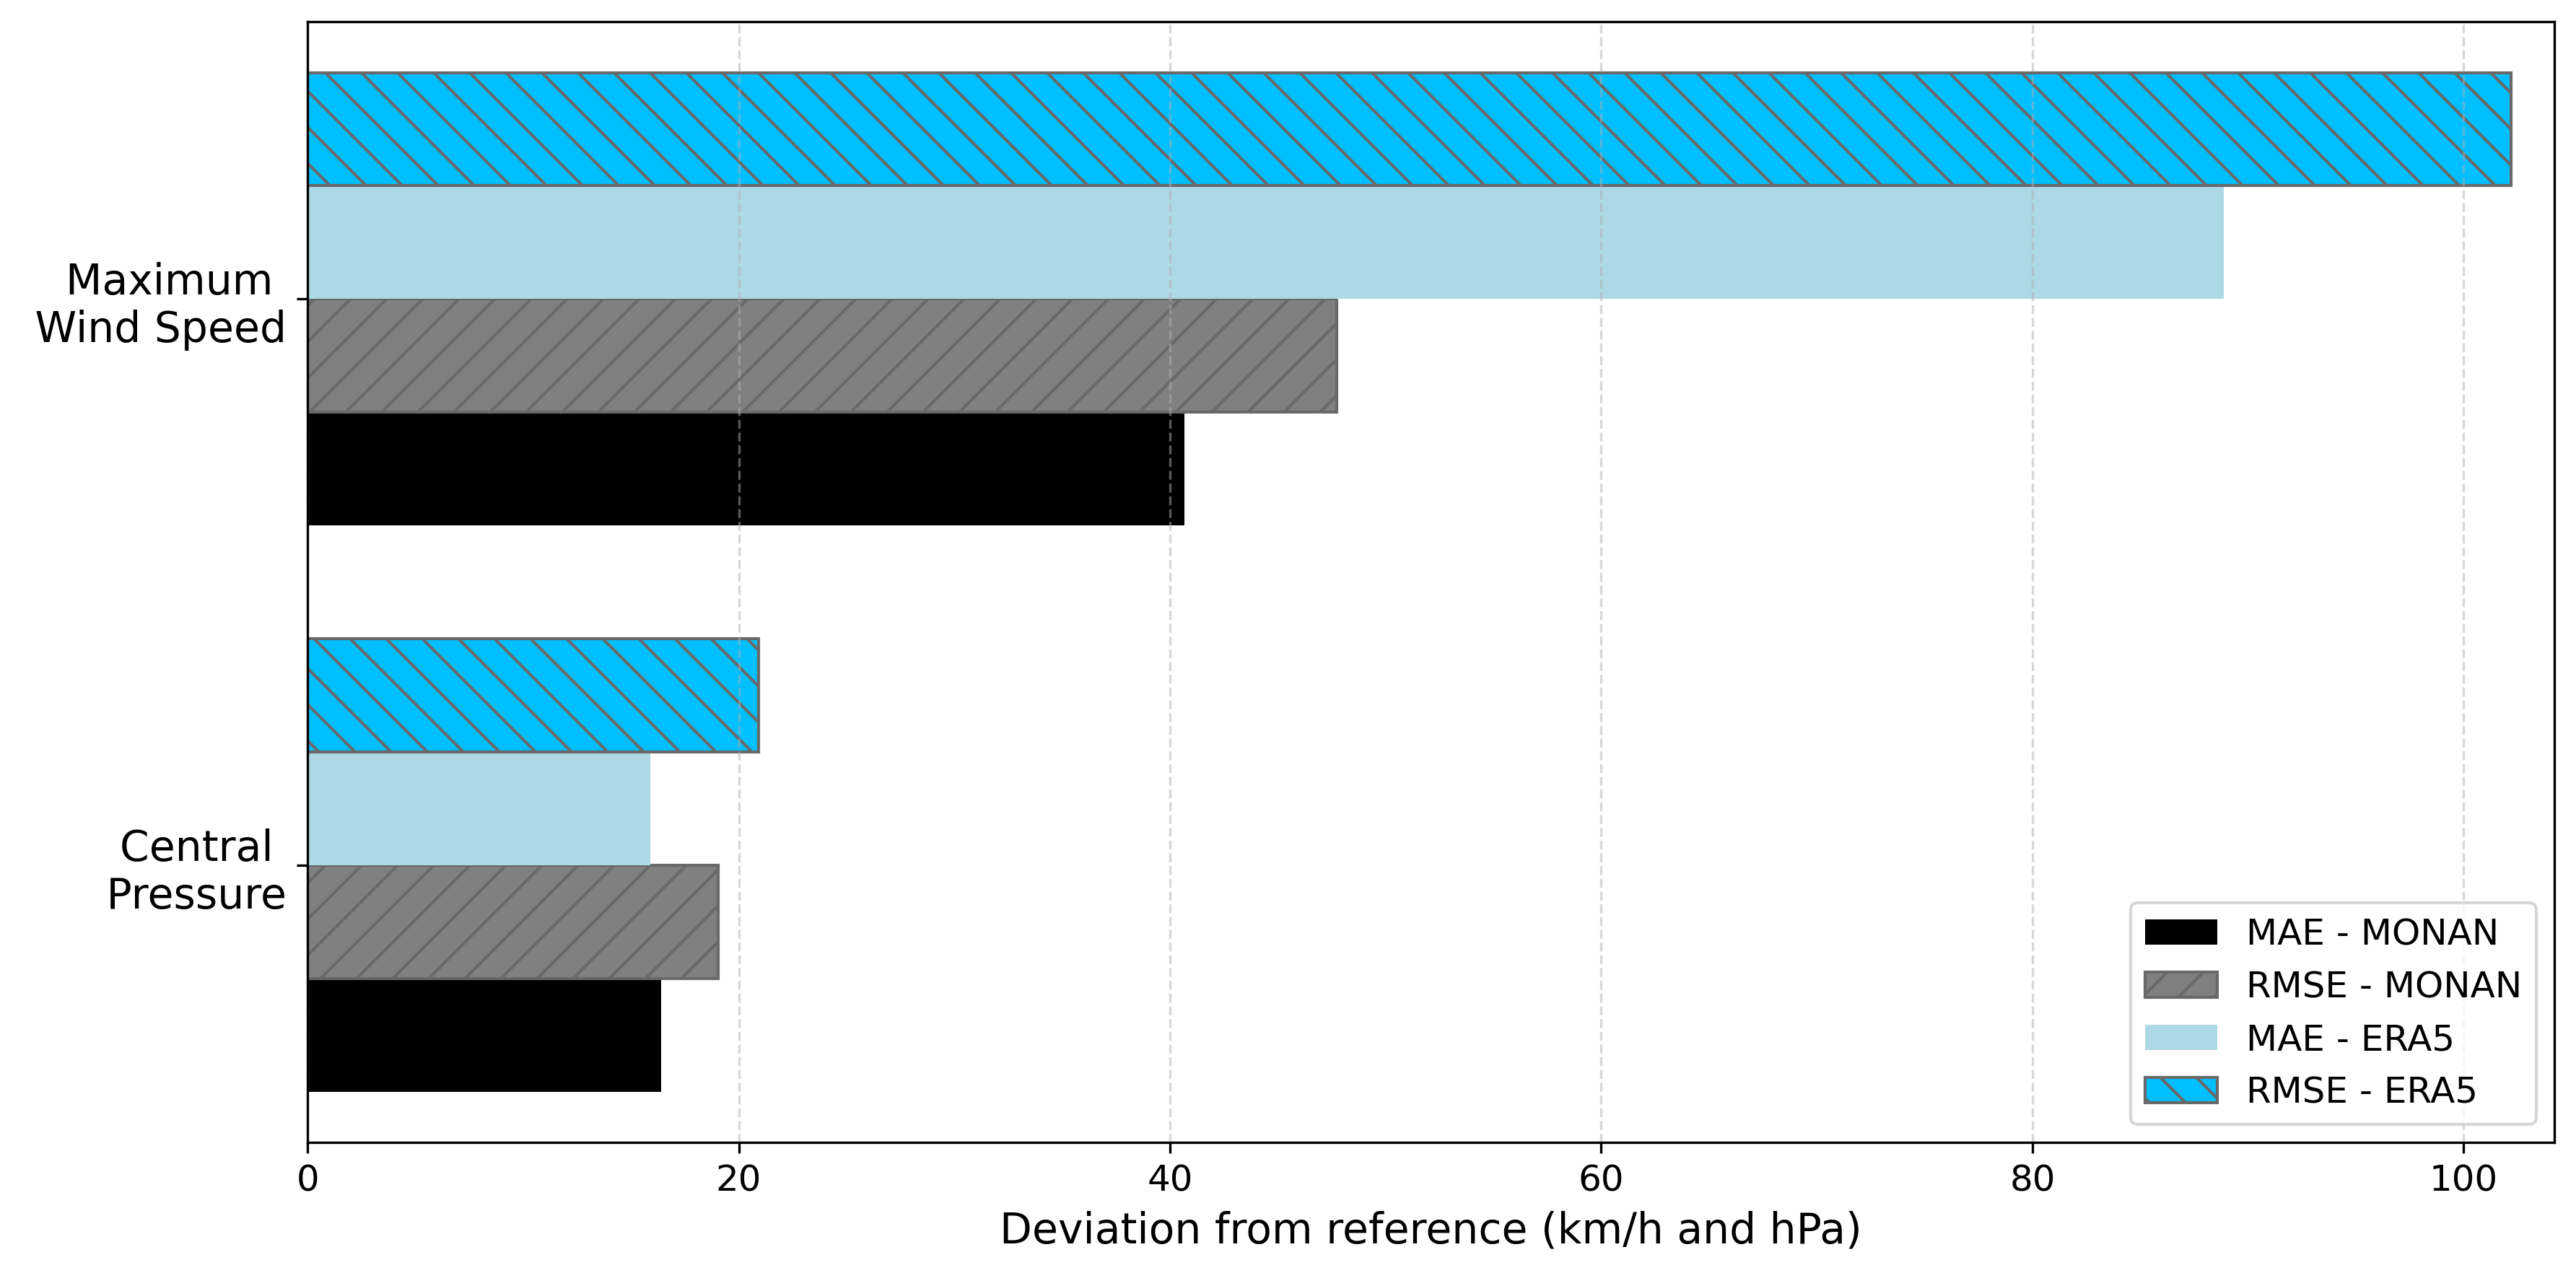
\includegraphics[width=\textwidth]{docs/figuras/chapter5/barplot_mean_error_monan_era5_intensity_FINAL.png} 
	\vspace{0.5em}
	Source: Made by the author (2025).  % Fonte abaixo da imagem
	\label{fig:errorsmona} % Label para referenciar no texto
\end{figure}

In contrast to the trajectory analysis, the advancements in the forecasting capabilities of MONAN are evident, particularly in the substantial reduction of maximum wind speed, which has decreased by approximately 54\% when compared to the ERA5 reanalysis.













